\documentclass[a4paper]{amsart}

\usepackage{graphicx}
\usepackage[colorlinks,urlcolor=blue]{hyperref}

\renewcommand{\baselinestretch}{1.15}
\setlength{\parskip}{3pt}

\title{Gemoetric point of view of p-integral}

\begin{document}
    \maketitle
    
    \noindent The following result is given in the lecture,
    \[ \int_{x=1}^{+\infty} x^{-p} \, dx =
        \begin{cases}
        \dfrac{1}{p-1}, \qquad &\text{if } p>1 \\[10pt]
        \text{diverges}, &\text{if } 0 < p \le 1.
        \end{cases} \]
    Once we have this, we can argue from a geometric point of view that $ \int_0^1 x^{-p} \, dx $ is symmetric to the above result.
    
    \begin{figure}[h]
    \centering
    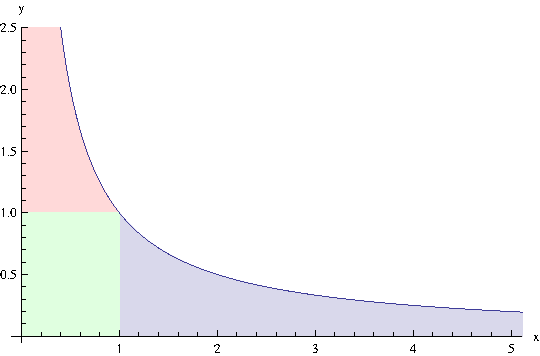
\includegraphics[width=0.7\linewidth]{p_integral_fig1}
    \caption{}
    \label{fig:p_integral_fig1}
    \end{figure}
    
    The blue area of figure 1 can depict the definite integral $ \int_{x=1}^{+\infty} x^{-p} \, dx $, whereas $ \int_0^1 x^{-p} \, dx $ can be interpreted as the sum of green and red area. The green area is finite and it equals one. This way, we can see that $ \int_0^1 x^{-p} \, dx $ converges if and only if the red area is finite.
    
    If we can exchange the $ x $-axis and the $ y $-axis and the red area becomes the blue area, then we can reduce the problem to one that is already solved. Simply view the screen as a paper and f{}lip (or mirror, reflect) the paper around the line $ y=x $. Another way to visualize the process is this. View the screen as an odd page in a book (odd pages are always right pages, see \href{https://en.wikipedia.org/wiki/Recto_and_verso}{recto and verso}), turn the page and rotate $ 90^\circ $ clockwise. You will get something like figure 2 on next page.
    
    We shall now view $ x $ as a function of $ y $ and the relationship is
    \begin{align*}
    y &= x^{-p} \\
    1/y &= x^p \\
    x &= y^{-1/p}.
    \end{align*}
    So the $ 1/p $ becomes the new $ p $. The red area converges if and only if $ 1/p > 1 $, this is the same as saying it converges if and only if $ p < 1 $. Moreover, when $ p < 1 $,  the sum of green area and red area is
        \[ 1 + \frac{1}{1/p-1} = 1 + \frac{p}{1-p} = \frac{1}{1-p}. \]
    Finally, we have
    \[ \int_0^1 x^{-p} \, dx =
        \begin{cases}
        \dfrac{1}{1-p}, \qquad &\text{if } 0 < p < 1 \\[10pt]
        \text{diverges}, &\text{if } p \ge 1.
        \end{cases} \]
        
    \begin{figure}[h]
        \centering
        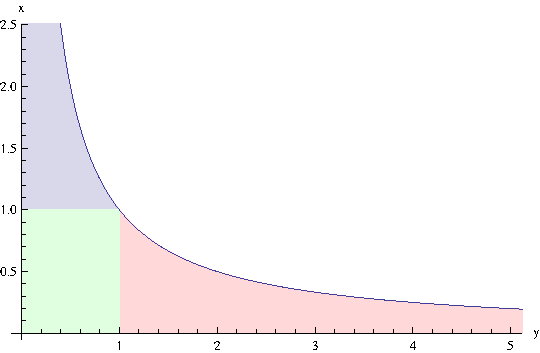
\includegraphics[width=0.7\linewidth]{p_integral_fig2}
        \caption{}
        \label{fig:p_integral_fig2}
    \end{figure}
    
\end{document}